\section{Non-Interactive Proofs of Proofs of Work}

\subsection{Sublinear SPV}
We would like to be able to prove statements like:

\begin{itemize}
  \item We have a valid chain where the last $k$ blocks are the ones we're
    claiming. This is called a \textbf{suffix proof}.
  \item We have a valid chain where a specific given block is included. This is
    called an \textbf{infix proof}.
\end{itemize}

Our current best solution, SPV, requires providing the whole chain's block
headers as proof. This is obviously linear in the size of the chain.

There have been previous attempts to create proofs smaller in size than SPV
proofs~\cite{KLS}, where a scheme for logarithmic proofs was proposed.
This scheme was later proven insecure~\cite{nipopows}.

NIPoPoWs is the first secure construction~\cite{nipopows} for logarithmic
proofs.

\subsection{Assumptions}
An assumption NIPoPoWs make is that the difficulty is constant. This is not
true for Bitcoin or Bitcoin Cash.

NIPoPoWs also assume each block contains an interlink data structure, which
we'll study shortly. Interlinks too don't exist in Bitcoin or Bitcoin Cash.

In the next section we'll look at how we sidestep all those issues.

\subsection{Levels}
At the heart of the primitive lies the separation of blocks into levels. The
level of a block is defined as $\textit{level}(B) = \left \lfloor \log(T) -
\log(\sf{id}(B)) \right \rfloor$, where $T$ is the constant difficulty of the
blockchain. The genesis block is an exception to this rule as
$\textit{level}(Gen) = \infty$. We call a block of level $\mu$ a $\mu$-superblock.

Intuitively, the level of a block is the number of leading zeros of the binary
representation of the block id when left padded to the length of $T$. An
example of this can be seen on Table~\ref{table:level-counting}.

\begin{table}
  \centering
  \begin{tabular}{|c|c|}
    \hline
    $T$ & 1110000 \\
    \hline
    $\sf{id}(B)$ & \underline{000}1000 \\
    \hline
  \end{tabular}
  \caption{Calculating the level of a block by counting the leading zeros (3 in this case).}
  \label{table:level-counting}
\end{table}

Figure~\ref{fig:hierarchy} shows an example the implied blockchain created from the superblocks.

\begin{figure}
  \centering
  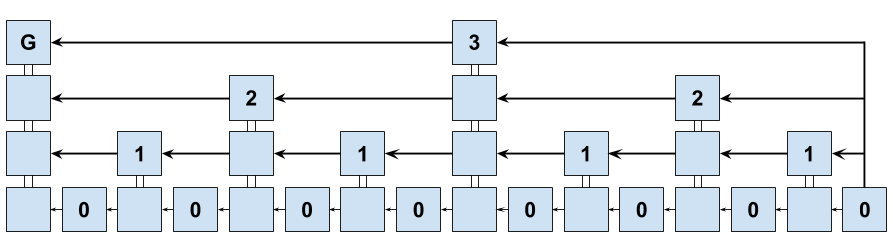
\includegraphics[width=0.9\columnwidth,keepaspectratio]{figures/hierarchical-ledger.png}
  \caption{The hierarchical blockchain.
  Higher levels have achieved a lower target (higher difficulty) during
  mining. All blocks are connected to the genesis block $G$. Source:~\cite{nipopows}}
  \label{fig:hierarchy}
\end{figure}

\subsection{Notation}
The NIPoPoWs paper introduces some notation for talking about blockchains with levels which we'll be using extensively. The notation is widely influenced by Python. Specifically:

\begin{itemize}
  \item $C$ denotes a blockchain, with $C[0]$ being the genesis block, $C[k]$ being the $k$-th first block and $C[-k]$ being the $k$-th last block.
  \item $C[k:]$ denotes the sub-blockchain starting from the $k$-th block, $C[-k:]$ denotes the sub-blockchain starting from the $k$-th last block.
  \item $C[:k]$ denotes the sub-blockchain ending before the $k$-th block, $C[:-k]$ denotes the sub-blockchain ending before the $k$-th last block.
  \item $C[i:j]$ denotes the sub-blockchain starting from the $i$-th block and ending at the $j$-th block. $i$ and $j$ can also be negative numbers similar to above.
  \item $C\upchain^\mu$ denotes the sub-blockset of C where all blocks are of level $\mu$ or higher.
\end{itemize}

\subsection{Interlink}
Instead of keeping only the hash of the previous block inside the block header,
for every superblock level we keep a pointer to the most recent superblock of that level. The structure
containing these pointers is called the interlink. Bitcoin does not support
such a structure in the block header but we will study how to sidestep this
issue by velvet forking in a few sections.

\begin{table}
  \centering
  \begin{tabular}{|c|c|}
    \hline
    Level & Block \\
    \hline
    $0$ & $C[-2]$ \\
    $1$ & $C[-2]$ \\
    $2$ & $C[-4]$ \\
    $3$ & $C[-8]$ \\
    $\infty$ & $C[0]$ \\
    \hline
  \end{tabular}
  \caption{Interlink of $C[-1]$ from Figure~\ref{fig:hierarchy}}
  \label{table:interlink-example}
\end{table}

It's important to note that the interlink can be encoded as a series of block ids, starting from $0$ up to $\infty$. It can also be compressed by using this series as the leafs of a Merkle tree and taking the Merkle tree root.

\subsection{Suffix Proofs}
\subsection{Infix Proofs}
\subsection{Proof Verification}
\subsection{Velvet Forks}
Velvet forks~\cite{nipopows,velvet} describe a formalization of adding
arbitrary data inside blocks in order to allow potential applications without
sacrificing the backwards compatibility of the blockchain. TODO

\subsection{User-Activated Velvet Forks}
